\section{Main comparison: performance on common coverage}
\label{sec:main-comparison}

Table~\ref{tab:main-comparison} reports, for every model and every date,
bid-ask coverage and median absolute implied-vol error on the COMMON
evaluation contract set (Sec.~\ref{sec:data}) -- SPX primary (all six
dates), AAPL secondary (held-out dates only, Table~\ref{tab:aapl-comparison}).
Each model's OWN additional coverage/exclusions beyond the common set are
reported separately in \texttt{report/data/full\_study\_results.json}
(dy2's \texttt{model\_masks}, solver convergence flags), never conflated
with the common-set numbers above.

\begin{table}[H]
\centering
\small
\begin{tabular}{lllll}
\toprule
Date & dy2 & SANOS snap. & DLV$\times$Black & DLV$\times$Bates \\
& \multicolumn{4}{c}{\% inside bid-ask / median abs IV err (bps)} \\
\midrule
2005-11-21 (sel.) & 96\% / 0.8bp & 96\% / 0.0bp & 10\% / 187.6bp & 100\% / 14.3bp \\
2010-07-07 (sel.) & 100\% / 6.7bp & 100\% / 0.7bp & 5\% / 310.0bp & 98\% / 43.9bp \\
\midrule
2011-07-07 & 98\% / 2.6bp & 100\% / 0.5bp & 12\% / 241.8bp & 94\% / 18.7bp \\
2024-03-05 & 100\% / 0.0bp & 100\% / 0.0bp & 0\% / 95.6bp & 20\% / 7.3bp \\
2024-12-26 & 91\% / 0.1bp & 100\% / 0.0bp & 0\% / 144.2bp & 27\% / 7.4bp \\
2025-01-03 & 87\% / 0.3bp & 100\% / 0.0bp & 4\% / 126.2bp & 13\% / 6.4bp \\
\bottomrule
\end{tabular}

\caption{SPX: bid-ask coverage and median absolute IV error by model and date. Held-out dates below the divider.}
\label{tab:main-comparison}
\end{table}

\begin{table}[H]
\centering
\small
\begin{tabular}{ll}
\toprule
Date & Status \\
\midrule
2011-07-07 & NOT RUN -- see note below \\
2024-03-05 & NOT RUN -- see note below \\
2024-12-26 & NOT RUN -- see note below \\
2025-01-03 & NOT RUN -- see note below \\
\bottomrule
\end{tabular}

\textbf{NOT RUN, exact reason}: every AAPL date failed with the identical error \texttt{`For live access to WIDB, set the environment variable WRDS\_USERNAME: currently not set.'}, raised inside \texttt{enrich\_day} (called from \texttt{mk\_arb\_free\_day} $\to$ \texttt{filter\_options\_day} $\to$ \texttt{smooth\_interpolated\_market}) -- a single-name dividend/borrow input is not present in the local fixture cache for this filter configuration (unlike SPX, an index with no dividend-forecast dependency), and its computation requires live WRDS access. \textbf{Exact fix}: a WRDS account with the Option Metrics entitlement, \texttt{WRDS\_USERNAME} set, and a \texttt{\textasciitilde/.pgpass} file (per \texttt{README.md}'s WRDS setup instructions) -- identical requirement already recorded in \texttt{DATA\_STATUS.md} from the prior task.
\caption{AAPL (secondary robustness check, held-out dates only).}
\label{tab:aapl-comparison}
\end{table}

\begin{figure}[H]
\centering
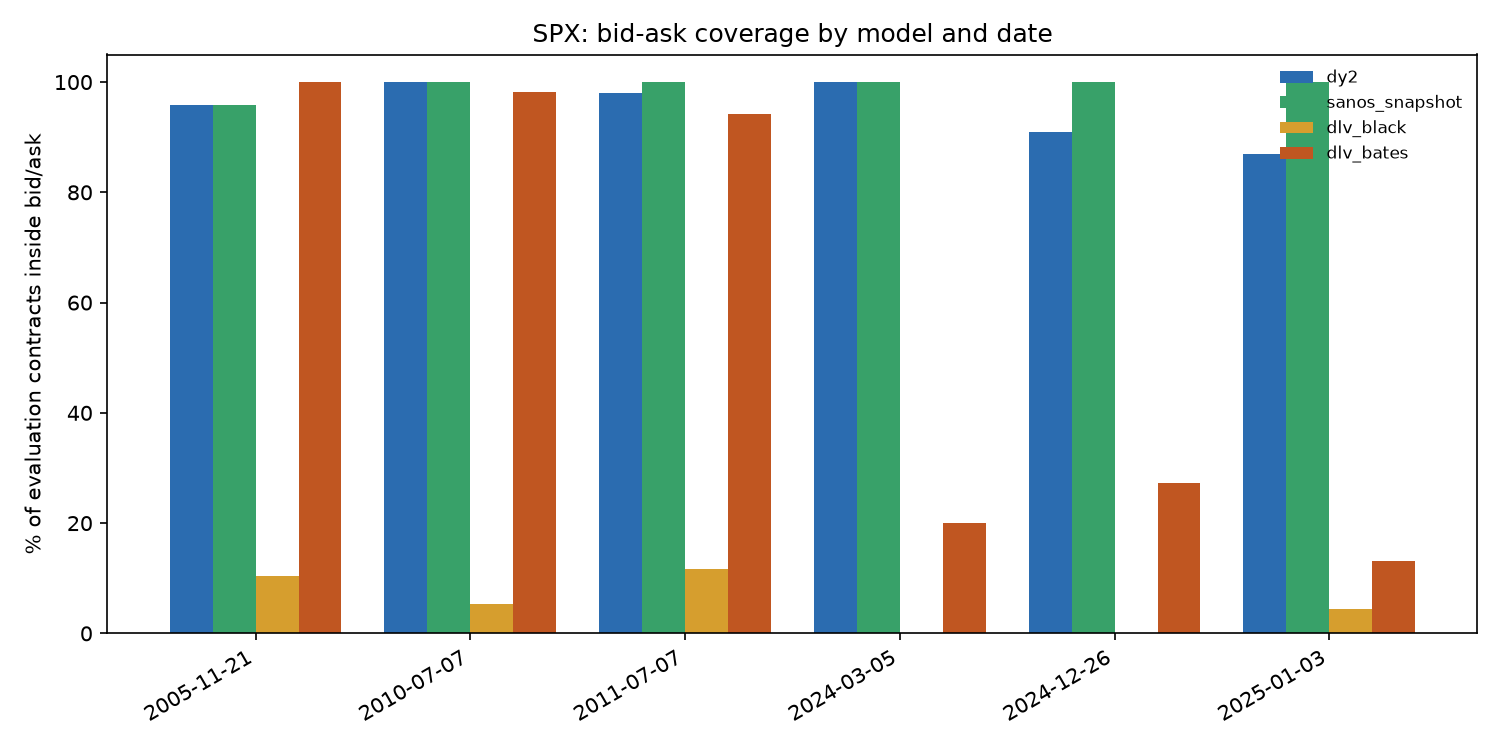
\includegraphics[width=\textwidth]{figures/model_comparison_bars.png}
\caption{SPX bid-ask coverage by model and date.}
\label{fig:model-comparison-bars}
\end{figure}

\begin{figure}[H]
\centering
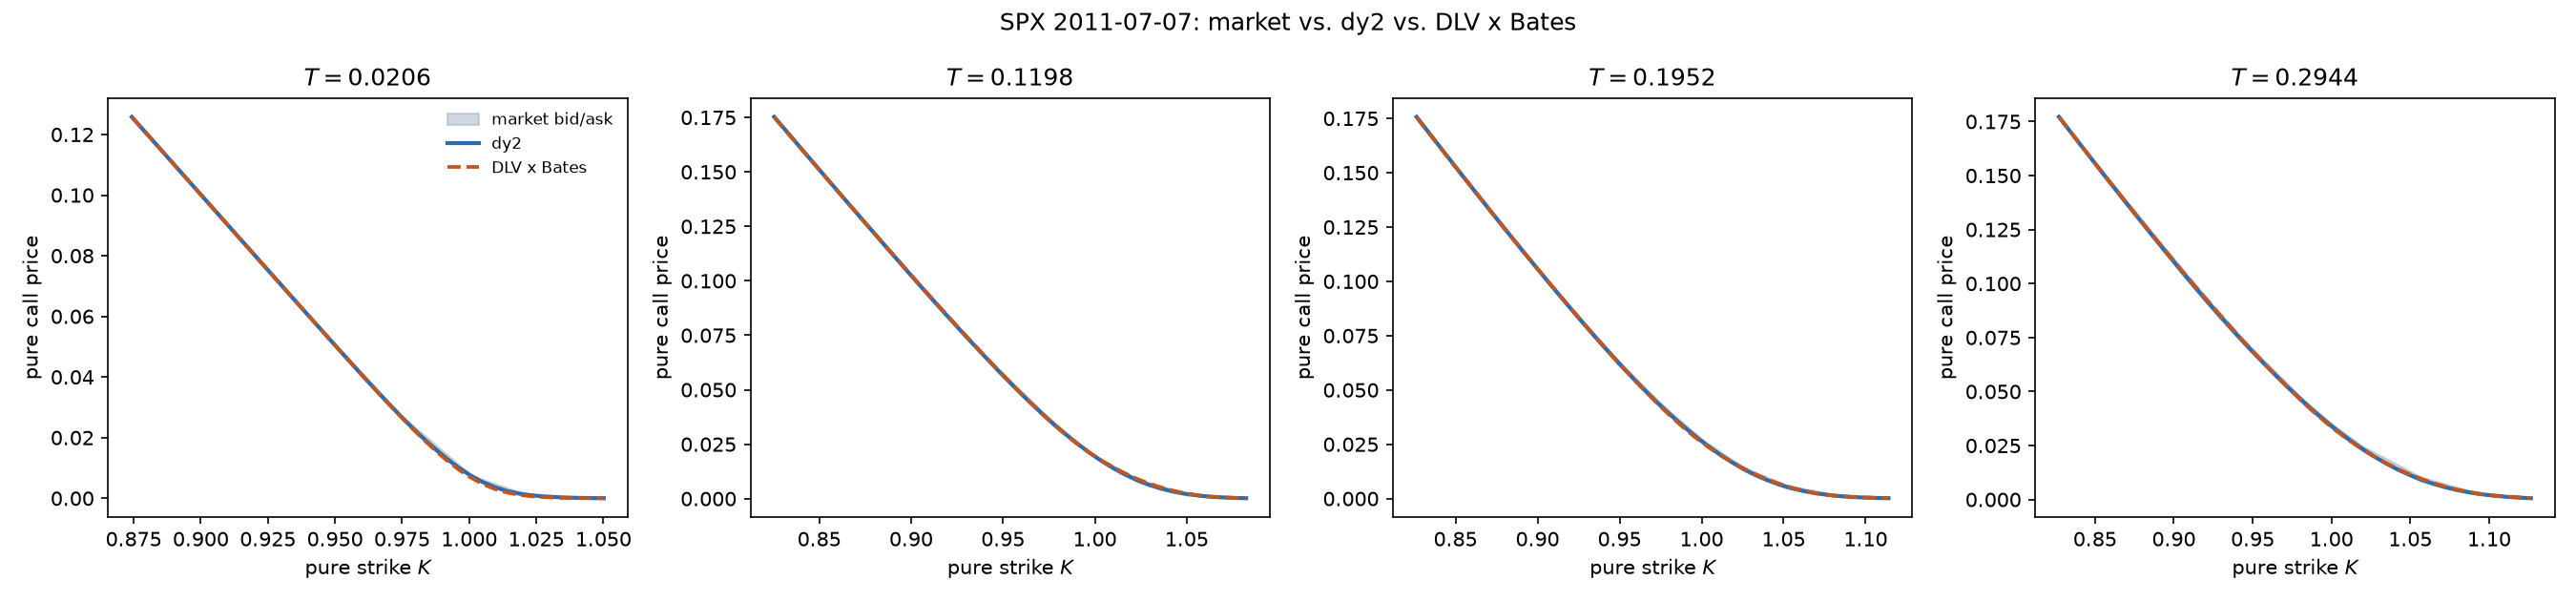
\includegraphics[width=\textwidth]{figures/surface_comparison_SPX_2011-07-07.png}
\caption{Market quotes vs.\ dy2 vs.\ DLV$\times$Bates, a representative held-out date.}
\label{fig:surface-comparison}
\end{figure}
